
\chapter{Linear Algebra Background}

%\chapterimage{Main/head1.png} % chapter 1

In this chapter we go through a quick overview of the mathematical foundations needed for a thorough study of deep learning. In Section \ref{vec-spaces} we recall the basics of vector spaces, norms, and linear maps. This leads us to the important concepts of eigenvalue and singular value decomposition in Section \ref{eig-sing}. 

% DID NOBODY DO THIS??
%In Section \ref{prob-theory} we review the basics of probability theory: random variables, probability distributions, expectation values, variance, and so on. Finally we conclude with Section \ref{optim} where we discuss some numerical computation techniques useful in the field of optimization. 

\section{Vector Spaces}\label{vec-spaces}

We assume the reader has some familiarity with linear algebra so we simply review some of the major concepts needed to proceed, often without proof. The main object of study in linear algebra is the vector space.

\begin{definition}
A \define{real vector space} is a triple $(V,+,\cdot)$ where $V$ is a set and

\begin{align*}
    +:V\times V\to V & \ \  \text{(\textit{vector addition})} \\
    \cdot\ :\R\times V\to V & \ \  \text{(\textit{scalar multiplication})}
\end{align*}
satisfy the following properties. For any $\vu, \vv, \vw \in V$ and $c, d \in \R$,
\begin{enumerate}
\item $\vu + \vv = \vv + \vu$ 
\item $(\vu + \vv) + \vw = \vu + (\vv + \vw)$ 
\item There exists $\vzero\in V$ such that $\vu + \vzero = \vu$ for any $\vu\in V$
\item For each $\vu \in V,$ there exists a vector $-\vu$ such that $\vu + (-\vu) = \vzero$
\item  $c(\vu + \vv) = c\vu + c\vv$
\item $(c+ d) \vu = c\vu + d\vu$
\item $c(d\vu) = (cd) \vu$
\item $1 \vu = \vu$
\end{enumerate}
\end{definition}

The most common vector space we will use is the space $\R^n$ of all $n$-tuples of real numbers, with $+$ and $\cdot$ defined point-wise. We take the convention that elements of $\R^n$ are column vectors:
$$\vx = \begin{bmatrix}x_1\\x_2\\\dots\\x_n\end{bmatrix}$$
but sometimes we may wish to save space and write them as row vectors:
$\vx = [x_1, x_2, \dots x_n]$ when no confusion can arise from doing so. In this notation we have $[x_1,\dots,x_n] + [y_1,\dots,y_n] = [x_1+y_1,\dots,x_n+y_n]$ and $r[x_1,\dots,x_n] = [rx_1,\dots,rx_n]$ for $r, x_1,\dots,x_n,y_1,\dots,y_n\in\R$. In other words, by convention we identify $\R^n$ with the matrix space $\R^{(n,1)}$ but for convenience may choose to identify $\R^n$ with $\R^{(1,n)}$ when it suits us (see Section \ref{matrix-section}). 

\subsection{Span, Linear Independence, Basis}

There is no preferred coordinate system in an abstract vector space. In order to prescribe meaningful coordinate representations of vectors, we need the concept of a basis. For this, we first need to discuss the concepts of linear independence and span.

\begin{definition}
The \textit{span} of $S = \{\vv_1, \ldots, \vv_n \} \subset V$ is the set 
$$\spann(S) := \{a_1\vv_1 + \ldots + a_k \vv_k : a_1,\dots,a_k \in \mathbb R \}$$
\end{definition}

\begin{example}
The typical well at a cocktail bar contains at least four ingredients at the bartender's disposal; vodka, tequila, orange juice, and grenadine. Assuming we have this well, we can represent drinks as points in $\mathbb R^4$, with one element for each ingredient. For instance, a tequila sunrise can be represented using the point 
$$[0, 1.5, 6, 0.75]^\intercal$$
representing amounts of vodka, tequila, orange juice, and grenadine (in ounces). The set of drinks can be represented as a subset of the span 
$$\spann(\{ [1,0,0,0]^\intercal, [0,1,0,0]^\intercal, [0,0,1,0]^\intercal,[0,0,0,1]^\intercal\})$$

(consisting of vectors with non-negative coefficients). Further, the bartender might be able to save time by making the observation that many drinks have the same orange juice - to - grenadine ratio, and therefore mix the two. So they might simplify their well by mixing the two: 
$$\spann(\{[1,0,0,0]^\intercal, [0,1,0,0]^\intercal, [0,0,6,0.75]^\intercal\})$$
Notice, it is now easier to pour drinks but this bartender can no longer make as many drinks, such as a screwdriver which contains orange juice but no grenadine.  
\end{example}

\begin{figure}[H]%
\centering
\subfigure[Span of one vector]{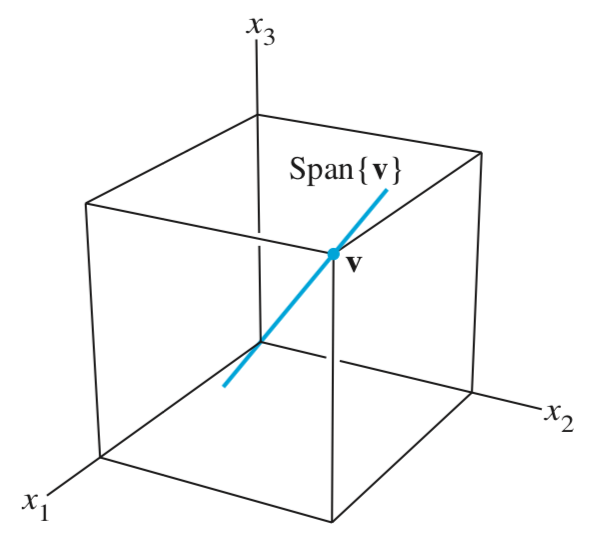
\includegraphics[width=5cm]{Chapter1/spanex1.png}}
\subfigure[Span of two vectors]{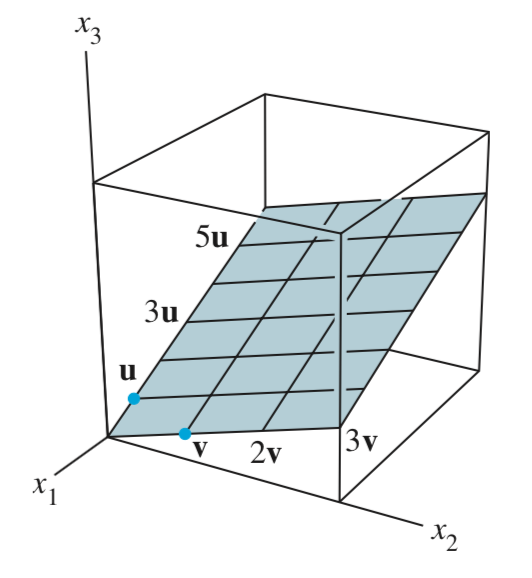
\includegraphics[width=4cm]{Chapter1/spanex2.png}}
\hfill
\caption{Linear Spans}
\end{figure}

\begin{definition}
A set $S \subset V$ of vectors is \define{linearly dependent} if there exists a non-empty linear combination of elements $\vv_k \in S$ yielding 
$$\sum_{k = 1}^m c_k \vv_k = 0$$
where $c_k \not = 0$ for all $k$. A set that is not linearly dependent is called \define{linearly independent.}
\end{definition}

\begin{definition}
The \define{dimension} of $V$ is the maximal size $|S|$ of a linearly independent set $S \subset V$ such that $\spann(S) = V.$
Any linearly independent set $S$ of maximal size $|S|$ with $\spann(S) = V$ is called a \define{basis} of $V$.
\end{definition}

\begin{example}
The standard basis for $\mathbb R^n$ is the set of vectors of the form 
$$\ve_k = [ \underbrace{0, \ldots, 0,}_{k - 1 \text{ elements}} 1, \underbrace{0, \ldots, 0}_{n - k \text{ elements}}]^\intercal$$
for $1\leq k\leq n$.
\end{example}

\subsection{Vector Norms}

One often needs the concept of length or distance when discussing vectors in a vector space. There are many different meaningful ways to define these concepts for a given vector space. To this end, we introduce vector norms.

\begin{definition}\label{norm-def}
A \define{vector norm} is a function $\norm{\cdot} : \R^n \rightarrow [0, \infty)$ satisfying the following conditions: 
\begin{enumerate}
\item $\norm{\vx} = 0$ if and only if $x = 0$ (Nondegeneracy)
\item $\norm{c\vx} = |c| \norm{\vx}$ for all scalars $c \in \R, \vx \in \R^n$ (Absolutely scalability) 
\item $\norm{\vx + \vy} \leq \norm{\vx} + \norm{\vy}$ for all $\vx,\vy \in \R^n$ (Triangle Inequality)
\end{enumerate}
\end{definition}

\begin{example}

For $p\geq 1$, $p\in\mathbb{Z}$ we define the \define{$p$-norm} on $\mathbb{R}^n$ by
\begin{equation}
    \norm{\vx}_p : = (|x_1|^p + |x_2|^p + \ldots + |x_n|^p)^{\frac{1}{p}}
\end{equation}
and the \define{infinity norm}
\begin{equation}
    \norm{\vx}_{\infty} : = \max (|x_1|, |x_2|, \ldots, |x_n|).
\end{equation}
We leave it to the reader to verify that these are indeed vector norms according to Definition \ref{norm-def}. One should observe that the limit as $p$ approaches infinity of the $p$-norms of a vector is equal to its infinity norm. The most common measure of length is the 2-norm. Given a norm $\norm{\cdot}$ one can define the distance between two vectors $\vx,\vy$ with respect to the norm $\norm{\cdot}$ as $\norm{\vx-\vy}$. The most commonly used distance is the 2-norm distance.
\end{example}

\begin{center}
  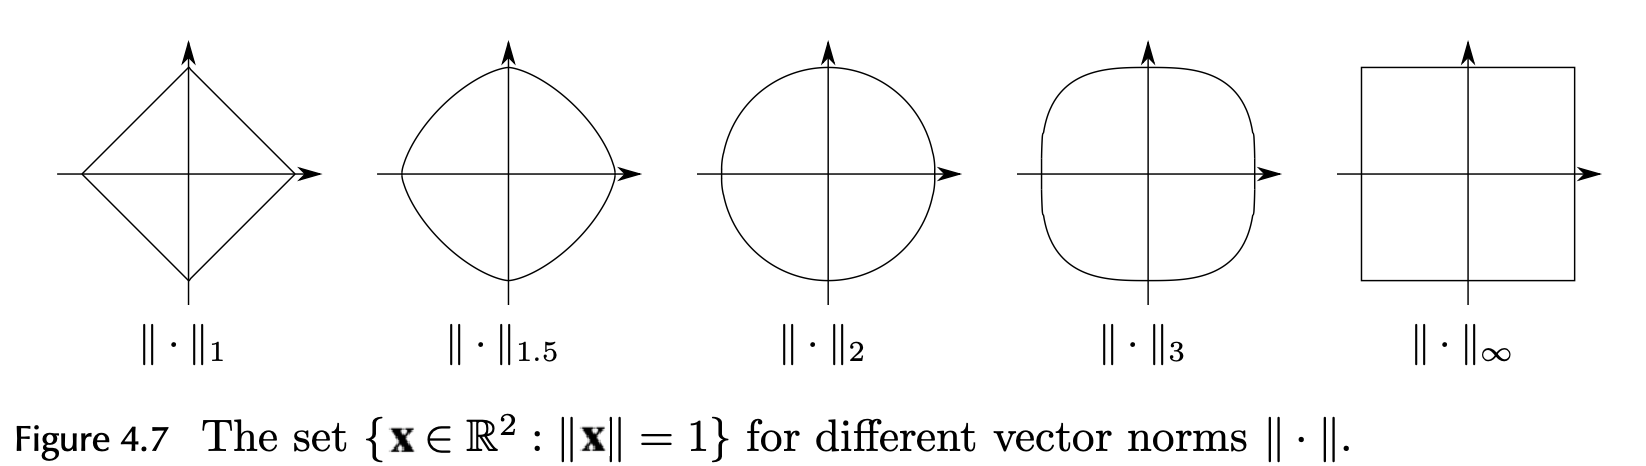
\includegraphics[width=6in]{Chapter1/norms.png}
\end{center}
%\textbf{Insert picture of the set } $\{x \in \mathbb R^2 : \norm{x} = 1\}$


Two norms $\norm{\cdot}$ and $\norm{\cdot}'$ are said to be equivalent if there exists constants $c_{\text{low}}$ and $c_{\text{high}}$ such that 
$c_{\text{low}} \norm{\vx} \leq \norm{\vx}' \leq c_{\text{high}} \norm{\vx}$
for all $\vx \in \mathbb R^n$. The equivalence theorem of norms in finite dimension tells us that all norms on $\mathbb R^n$ are equivalent. We leave it to the reader to seek a proof of this surprising fact, if desired.

\section{Linear Maps}

It is a pervasive concept in mathematics that in order to understand a given class of objects, one must study the maps between such objects which preserve the defining structure of the objects. In our case, this leads us to the study of linear maps.

\begin{definition}\label{linear-def}
Suppose $V$ and $V'$ are vector spaces. Then a mapping $T : V \rightarrow V'$ is \define{linear} if it satisfies the following for all $\vv_1, \vv_2 \in V$ and $c \in \mathbb C$:
\begin{itemize}
\item $T(\vv_1 + \vv_2) = T(\vv_1) + T(\vv_2)$
\item $T(c\vv) = c T(\vv)$
\end{itemize}
\end{definition}

\begin{example}\label{lin-map-ex}
Consider the map $T : \mathbb R^2 \to \mathbb R^3$ defined by
$T([x,y]^\intercal)=[3x, 2x + y, -y]^\intercal$.
More generally, let $A\in\mathbb{R}^{m\times n}$ be a matrix and define a map $T_A:\mathbb{R}^n\to\mathbb{R}^m$ by $T_A(x)=Ax$. 
We leave it to the reader to verify these maps are indeed linear according to Definition \ref{linear-def}. 
\end{example}

\begin{proposition} 
A linear mapping $T$ on $\mathbb R^n$ is completely determined by its action on the standard basis vectors $\ve_k.$
\end{proposition}

\begin{proof} For any $\vv\in\R^n$ we have
$$
T(\vv) = 
T(\sum_{k } v_k \ve_k) = 
\sum_k T(v_k \ve_k) = 
\sum_k v_k T(\ve_k)\qedhere
$$
\end{proof}

\begin{example}
Returning the previous example: 

$$T([x,y]^\intercal) = x T(\ve_1) + y T(\ve_2) = x [3,2,0]^\intercal
+ y [0,1,-1]^\intercal. $$
\end{example}

\subsection{Matrices}\label{matrix-section}

Once we choose bases, linear maps between vector spaces can be represented by 2-dimensional arrays called matrices. Linear maps are often easier to study by thinking about the matrices which represent them. 

\begin{definition}
The \define{space of matrices} $\mathbb R^{m \times n}$ is the set composed of matrices of the form: 
$$
\MV =
\begin{bmatrix}
V_{11} & V_{12} & \ldots & V_{1n} \\
V_{21} & V_{22} & \ldots & V_{2n} \\
\vdots & \vdots & \ddots & \vdots \\
V_{m1} & V_{m2} & \ldots & V_{mn} \\
\end{bmatrix} $$
with $V_{i,j} \in \mathbb R$ for $1\leq i\leq m$ and $1\leq j\leq n$. For $1\leq i\leq m$ we let $\MV_{i,*} = [V_{i,1},\dots,V_{i,n}]^\intercal$ denote the $i$th row of $\MV$ and for $1\leq j\leq n$ we let $\MV_{*,j} = [V_{1,j},\dots,V_{m,j}]^\intercal$ denote the $j$th column of $\MV$. We follow the common convention that both are interpreted as column vectors.
\end{definition}

\begin{definition}
Matrix to vector multiplication is defined by 
$$\begin{bmatrix}
\vdots & \vdots & \ldots & \vdots \\
\MV_{*,1} & \MV_{*,2} & \ldots & \MV_{*,n} \\
\vdots & \vdots & \ldots & \vdots \\
\end{bmatrix} \begin{bmatrix}
c_1 \\
c_2 \\
\vdots \\
c_n
\end{bmatrix} = c_1 \MV_{*,1} + c_2 \MV_{*,2} + \ldots + c_n \MV_{*,n}.$$
\end{definition}

The Riesz representation theorem links the concepts of linear mappins with matrices. Riesz states that any linear map can be expressed as matrix to vector multiplication by a fixed matrix (once a basis is picked for both the domain and codomain).

\begin{theorem}[Riesz Representation] Every linear mapping from a vector space $V$ to $V'$, there exists a unique linear matrix $A$ (up to a chosen bases on the domain and codomain) such that 
$$T\left(\begin{bmatrix}x \\ \vdots \\ y\end{bmatrix}\right) = A \begin{bmatrix}x \\ \vdots \\ y\end{bmatrix}$$
\end{theorem}

\begin{example}
The linear map $T$ from Example \ref{lin-map-ex} can be written 
$$T\left(\begin{bmatrix}x \\y\end{bmatrix}\right) 
= 
\begin{bmatrix}
3 & 0 \\
2 & 1 \\
0 & -1
\end{bmatrix} 
\begin{bmatrix}
x \\
y
\end{bmatrix}$$
\end{example}

In many ways, this theorem is profound. If you want to define a linear function from $\mathbb R^3$ to $\mathbb R^{100000000000000}$, you simply have to define exactly 3 points, each corresponding to the evaluation of the function on each of the basis vectors. In the context of machine learning, this theorem provides us a one-to-one correspondence to represent every (linear) function simply as an array. 

\begin{definition}
Matrix to matrix multiplication is defined by natural extension of matrix to vector multiplication
$$\MM \begin{bmatrix}
\vdots & \vdots & \ldots & \vdots \\
\vv_1 & \vv_2 & \ldots & \vv_n \\
\vdots & \vdots & \ldots & \vdots \\
\end{bmatrix} = \begin{bmatrix}
\vdots & \vdots & \ldots & \vdots \\
\MM \vv_1 & \MM \vv_2 & \ldots & \MM\vv_n \\
\vdots & \vdots & \ldots & \vdots \\
\end{bmatrix}$$
\end{definition}

A matrix $\MA\in\R^{n\times n}$ is said to be \define{invertible} if there exists a matrix $\MB\in\R^{n\times n}$ such that $\MA\MB = \MI = \MB\MA$ where $\MI$ is the identity matrix ($I_{i,j}$ is $1$ if $i=j$ and $0$ otherwise). In this case one will write $\MB = \MA^{-1}$.

\begin{example}
Returning to the cocktail example, suppose we make two drinks from our 3 defined wells of liquid (vodka, tequila, and the mix of grenadine and orange juise). Then to find the basic ingredients we simply use matrix multiplication: 

$$ \begin{bmatrix}
1 & 0 & 0 \\
0 & 1 & 0 \\
0 & 0 & 6 \\
0 & 0 & 0.75
\end{bmatrix}\begin{bmatrix}
0 & 0.75 \\
1.5 & 0.75 \\
1 & 2 
\end{bmatrix} = \begin{bmatrix}
0 & 0.75 \\
1.5 & 0.75 \\
6 & 12 \\
0.75 & 1.5
\end{bmatrix}$$
\end{example}

\subsection{Some Common Matrix Operations} 

In this section we introduce the transpose, trace, induced matrix norm, and determinant, along with some useful properties of the common operations.

\begin{definition}\label{trans-def}
The \define{transpose} of a matrix $\MA \in \mathbb R^{m \times n}$ is the matrix $\MA^\intercal \in \mathbb R^{n\times m}$ with elements defined by 
$$A^\intercal_{i,j} = A_{j,i}$$ 
for all $1\leq i\leq m$ and $1\leq j\leq n$.
\end{definition}

\begin{definition}
The \define{trace} of a matrix $\MA$ is $\trace(\MA) = \sum_i \MA_{ii}$.
\end{definition}

The reader can verify that for all matrices $\MA,\MB$ we have
\begin{enumerate}
    \item $(\MA^\intercal)^\intercal = \MA$
    \item $(\MA + \MB)^\intercal = \MA^\intercal + \MB^\intercal$
    \item $(\MA\MB)^\intercal = \MB^\intercal \MA^\intercal$
    \item $\trace(\MA) = \trace(\MA^\intercal)$
    \item $\trace(\MA\MB) = \trace(\MB\MA)$
\end{enumerate}

We found norms to be a useful operation on vectors, and we would like to bootstrap that construction to get a similar operation on matrices.

\begin{definition}
The \define{induced matrix norm on} $\mathbb R^{m \times n}$ by a vector norm $\norm{\cdot}$ is given by 
$$\norm{\MA} = \max_{\norm{\vx} = 1} \norm{\MA\vx}.$$
\end{definition}

\begin{figure}
\centering
  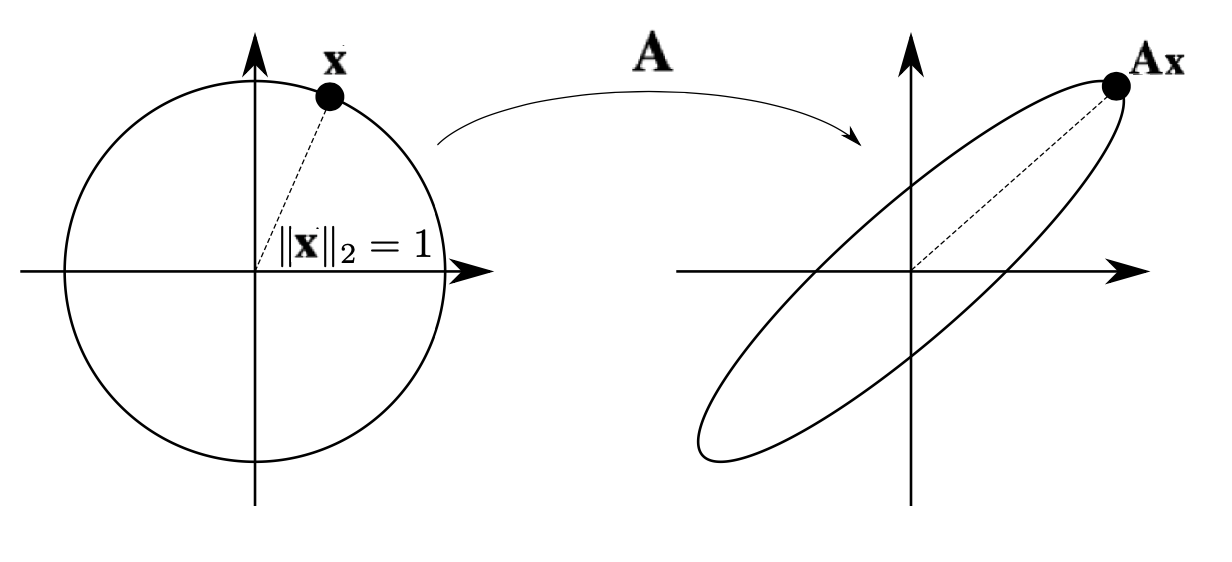
\includegraphics[width=3.5in]{Chapter1/induced_norm.png}
  \caption{This figure illustrates the intuition of the matrix norm of a 2 by 2 matrix $\MA$. We simply look at the image of the unit circle and find the distance of the point furthest from the origin.}
\end{figure}

\begin{example}
    The reader may wish to prove the following as an exercise:
    \begin{enumerate}
        \item $\norm{\MA}_1 = \max_{1 \leq j \leq n} \sum_{i = 1}^m |A_{i,j}|$
        \item $\norm{\MA}_{\infty} = \max_{1 \leq i \leq m} \sum_{j = 1}^n |A_{i,j}|$
    \end{enumerate}
    In general, the $p$-norm has no such formula, but we will find soon that the SVD gives a nice way to compute the 2-norm.
\end{example}

Another useful norm for matrices is given by treating a matrix as if it were a vector and simply taking the vector norm.

\begin{definition}
The \define{Frobenius norm} is defined by
$\norm{\MA}_\Fro := \sqrt{\sum_{i,j} A_{i,j}^2}$.
\end{definition}

\begin{note}
The Frobenius norm cannot be induced from a vector norm.
\end{note}

The Frobenius norm has a useful relationship to the trace and transpose operations discussed previously.

\begin{proposition}
For any matrix $\MA$ we have
$$\norm{\MA}_\Fro  = \sqrt{\trace(\MA^\intercal\MA)}.$$
\end{proposition}

% \begin{definition}
% Given a positive definite matrix $A$, we can define a vector norm $\norm{\cdot}_A$ by 
% $$\norm{x} = \sqrt{x^\intercal A x}$$
% \end{definition}

Here we introduce the determinant of a matrix. We skip any motivation for the definition and simply write it down along with a few common consequences. The reader can consult any linear algebra textbook for more details.

\begin{definition}
Given a matrix $\MA \in \mathbb R^{n \times n}$, the \define{determinant} of $\MA$ is
$$\det(\MA) = \sum_{\pi \in \FS_n} (-1)^{\inv(\pi)} \prod_i A_{i, \pi(i)}$$
where $\FS_n$ is the set of permutations on $\{1,\dots,n\}$ and $\inv(\pi)$ is the number of inversions of $\pi$, that is, the number of pairs $i<j$ such that $\pi(i)>\pi(j)$.
\end{definition}

\begin{example}
For $n=2$ there are two permutations $(1,2)$ and $(2,1)$ on the set $\{1,2\}$ and we have $\inv(1,2) = 0$ and $\inv(2,1) = 1$. We find that
$$\det \left (\begin{bmatrix} 1 & 2 \\
3 & 4 \end{bmatrix} \right )  = 1\cdot4 - 3\cdot2 = -2.$$
\end{example}


\begin{note}
The geometric interpretation of the determinant is that it is the ratio volume of the image of the unit sphere after the action by the matrix $A$ divided by the volume of the unit sphere within the ambient vector space. There is a minus sign involved if the transformation reverses the orientation of the sphere.
\end{note}

 \begin{center}
  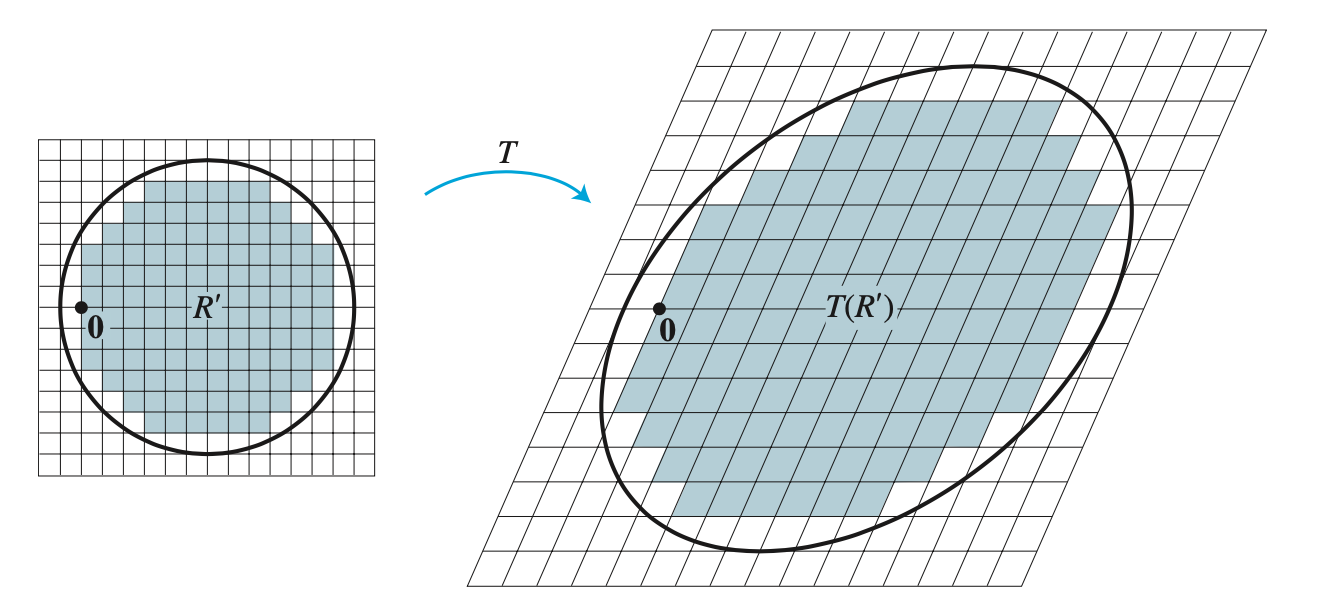
\includegraphics[width=3.5in]{Chapter1/det_stretch.png}
\end{center}

We state without proof that for any matrices $\MA,\MB$ of compatible dimensions, that

\begin{equation}
    \det(\MA\MB) = \det(\MA) \det(\MB).
\end{equation} 
We encourage the reader to seek out a proof of this fundamental result, along with the fact that a matrix has nonzero determinant if and only if that matrix is invertible.

\subsection{Orthogonality and The Inner Product Space \texorpdfstring{$\R^n$}{Rn}}

One of the most important constructions we are leading towards is the singular value decomposition (SVD) of a matrix. In order to define the SVD, we need the concept of orthogonality.

\begin{definition}
The \define{dot product} of two vectors $\vu$ and $\vv$ in $\R^n$ is given by 
$$\vu \cdot \vv = \vu^\intercal \vv.$$
\end{definition}

\begin{example}In $\mathbb R^2,$ we see 
$$[1,2]^\intercal \cdot [-2,6]^\intercal = 10$$
\end{example}

Notice that for $\vu\in\R^n$ we have
$\norm{\vu}_2 = \sqrt{u_1^2 + \ldots + u_n^2 } = \sqrt{\vu \cdot \vu}$. Geometrically, we may remember the following relationship: 
$$\vu \cdot \vv = \norm{\vu}_2 \norm{\vv}_2 \cos \theta$$

where $\theta$ is the angle between $\vu$ and $\vv$. When $\cos \theta = 0,$ we see that the dot product is also zero. This motivates the following definition: 

\begin{definition}Two vectors $\vu,\vv \in \mathbb R^n$ are \define{orthogonal} when $\vu \cdot \vv = 0.$
A set of vectors $\vv_1, \ldots, \vv_k$ is \define{orthonormal} if $\norm{\vv_i}_2 = 1$ for all $i$ and $\vv_i \cdot \vv_k = 0.$
A square matrix whose columns are orthonormal is called an \define{orthogonal matrix.}
\end{definition}

\begin{proposition}
A matrix $\MQ$ is orthogonal if and only if $\MQ$ is invertible and $\MQ^{-1} = \MQ^\intercal.$
\end{proposition}
\begin{proof}
This follows immediately from the definition of orthogonal matrix. The reader should write out the details as an exercise.
\end{proof}
 
\begin{definition}An \define{isometry} on $\mathbb R^n$ is a distance preserving bijection $f : \mathbb R^n \rightarrow \mathbb R^n$. That is, 
$$\norm{f(\vx) - f(\vy)}_2 = \norm{\vx - \vy}_2.$$
\end{definition}

\begin{center}
  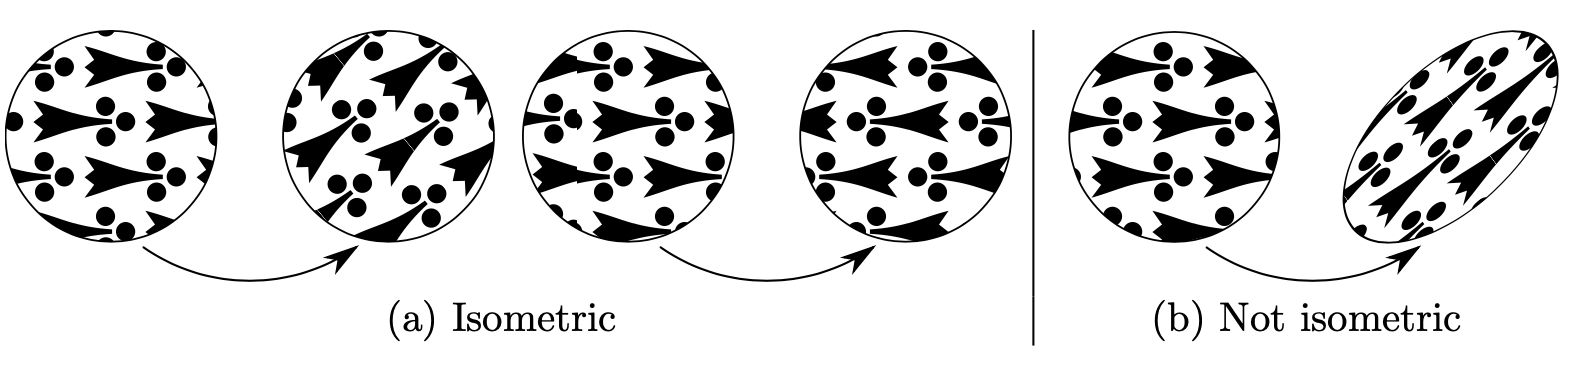
\includegraphics[width=4in]{Chapter1/isometric.png}
\end{center}

We end this section by stating without proof two commonly used facts about orthogonal matrices.

\begin{proposition}\ 
\begin{enumerate}
    \item If $\MQ$ is orthogonal, then the function $\vx \mapsto \MQ\vx$ is an isometry on $\mathbb R^n.$
    \item Every isometry on $\mathbb R^n$ can be written as $\vx \mapsto \MA + \MQ\vx$ for some $\MA, \MQ \in \mathbb R^{n \times n}$ with $\MQ$ orthogonal.
\end{enumerate}

\end{proposition}

\section{Eigenvalue and Singular Value Decompositions}\label{eig-sing}

Square matrices are often best understood by writing down a special decomposition called the eigenvector decomposition. To this end we define eigenvectors and eigenvalues. We will find especially nice decompositions for symmetric matrices.

\subsection{Eigenvalues and Eigenvectors} 

\begin{definition}
An \define{eigenvector} of a matrix $\MA \in \mathbb R^{n \times n}$  is a nonzero vector $v$ such that $\MA\vv = \lambda \vv$ for some scalar $\lambda. $ A scalar $\lambda$ is called an \define{eigenvalue} of $\MA$ if there is a nonzero vector $\vv$ such that $\MA\vv = \lambda \vv.$ 
\end{definition}

\begin{center}
  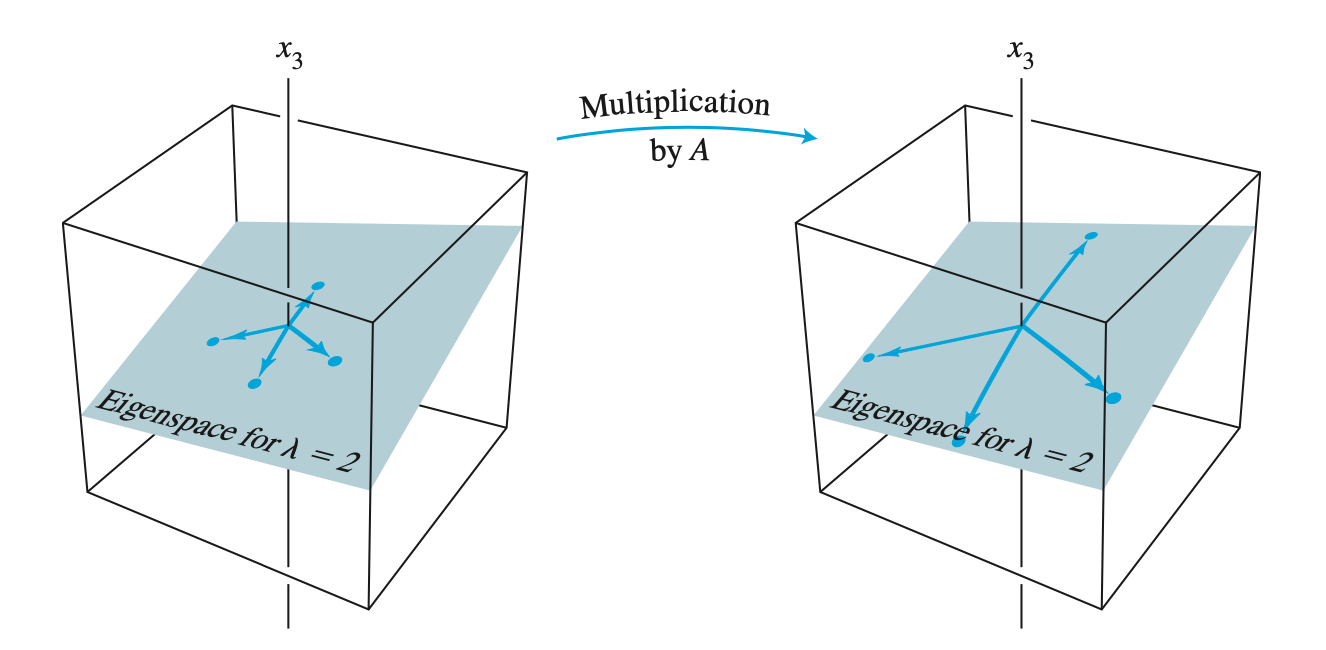
\includegraphics[width=4in]{Chapter1/invarient_space.png}
\end{center}

\begin{proposition}
Every matrix $\MA \in \mathbb R^{n \times n}$ has at least one (potentially complex) eigenvector. 
\end{proposition}
\begin{proof}
Take any vector $x \in \mathbb R^n \setminus \{ \vzero\} $ and assume $\MA \not = \vzero$ since this matrix trivially has eigenvalue 0. The set 
$\{\vx, \MA\vx, \MA^2 \vx, \ldots, \MA^n \vx\}$
must be linearly dependent because it contains $n + 1$ vectors in $n$ dimensions. So there exists constants $c_0, \ldots, c_n \in \mathbb R$ not all zero such that 
$\vzero = c_0 \vx + c_1 \MA\vx + c_2 \MA^2\vx + \ldots +c_n \MA^n \vx$.
We define the polynomial 
$f(z) = c_0 + c_1 z + \ldots + c_n z^n$
By the fundamental theorem of Algebra, there exist $m \geq 1$ roots $z_i \in \mathbb C$ and $c \not = 0$ such that 
$f(z) = c(z- z_1) (z - z_2) \ldots (z - z_m).$
Applying this factorization, we see that 
$
\vzero = c_0 \vx + c_1 \MA\vx  + \ldots +c_n \MA^n \vx =  c (\MA - z_1 \MI) \ldots (\MA - z_m  \MI) \vx.
$
In this form, at least one $\MA - z_i \MI$ has a null space, since otherwise each term would be invertible, forcing $\vx = \vzero,$ which we already assumed against. So if we take $\vv$ to be a nonzero vector in the null space of $\MA - z_i \MI,$ then by construction 
$\MA\vv = z_i \vv.$
\end{proof}


We recall here some basic facts one should be aware of, which hopefully the reader has seen in a previous course in linear algebra. Suppose $V$ is a complex vector space and $T:V\to V$ is a linear map. Let $\lambda_1, \ldots, \lambda_m$ denote the distinct eigenvalues of $T$, with multiplicities $d_1, \ldots, d_m$. Then the polynomial 
$$(z - \lambda_1)^{d_1} \ldots, (z - \lambda_m)^{d_m}$$
is called the \define{characteristic polynomial} of $T$. 
A scalar $\lambda$ is an eigenvalue of and $n \times n$ matrix $A$ if and only if $\lambda$ satisfies the characteristic equation 
$\det(A - \lambda I) = 0$.
The eigenvectors corresponding to distinct eigenvalues of a given matrix are linearly independent.
To understand why this is true,
suppose otherwise. Then there exists eigenvectors $\vv_1, \ldots, \vv_k$ with distinct eigenvalues $\lambda_1, \ldots, \lambda_k$ that are linearly dependent. This implies that there are coefficients $c_1, \ldots, c_k$ not all zero such that 
$\vzero = c_1 \vv_1 + \ldots + c_k \vv_k$. 
Notice, for any $i \not = j,$ we see that 
$(\MA - \lambda_i \MI) x_j = \MA\vx_j - \lambda_i \vx_j = (\lambda_j - \lambda_i) \vx_j$
We can then isolate one of the coefficients 
$\vzero = (\MA - \lambda_2 \MI) \ldots (\MA - \lambda_k \MI)c_1 \vv_1 + \ldots + c_k \vv_k = c_1 (\lambda_1 - \lambda_2) \ldots (\lambda_1 - \lambda_k) $
Since $\lambda_1$ does not equal any of the other distinct eigenvalues, then 
$c_1 = 0$
We can repeat this for all the either eigenvalues. 


\subsection{Symmetric and Positive Semi-definite Matrices}

Here we recall some facts and definitions about symmetric and positive (semi)-definite matrices. 
Recall a square matrix $\MA$ is \define{symmetric} if $\MA = \MA^\intercal.$ 
A symmetric matrix $\MA \in \R^{n \times n}$ is \define{positive semi-definite} if for every $\vx \in \R^n$ it follows that $\vx^\intercal \MA \vx \geq 0$, and is called \define{positive definite} if furthermore the only vector $\vx$ with $\vx^\intercal\MA\vx = 0$ is the zero vector $\vx =\vzero$.


\begin{theorem}\ 
\begin{enumerate}
    \item All eigenvalues of symmetric matrices are real. 
    \item Eigenvectors corresponding to distinct eigenvalues of symmetric matrices are orthogonal.
    \item If $A$ is positive-semidefinite, then $A$ has nonnegative real eigenvalues.
    \item If $A$ is positive-definite, then $A$ has positive eigenvalues.
    \item For any $\MA \in \R^{m \times n},$ the matrix $\MA^\intercal \MA$ is positive semidefinite. 
    \item For any $\MA \in \R^{m \times n},$ the matrix $\MA^\intercal \MA$ is positive definite provided the columns of $\MA$ are linearly independent. 
\end{enumerate}
\end{theorem}

\subsection{Diagonalization and Spectral Theorem}


A matrix $\MA \in \mathbb R^{n \times n}$ is said to be \define{diagonalizable} if $\MA = \MP\MD\MP^{-1}$ for some invertible matrix $\MP \in \mathbb R^{n \times n}$ and some diagonal matrix $\MD \in \mathbb R^{n \times n}$. 


\begin{theorem}
An $n \times n$ matrix $\MA \in \mathbb R^{n \times n}$ is diagonalizable if and only if $\MA$ has $n$ linearly independent eigenvectors. In this case, 
$\MA = \MP\MD\MP^{-1}$
where the columns of $\MP$ are exactly the eigenvectors of $\MA$ and the diagonal entries of $\MD$ are the eigenvalues of $\MA$. 
\end{theorem}

\begin{theorem}[Spectral Theorem]\label{thm-spec}
Suppose $\MA \in \C^{n \times n}$ is symmetric. Then $\MA$ has exactly $n$ orthonormal real eigenvectors $\vv_1, \ldots, \vv_n$ with (possibly repeated) eigenvalues $\lambda_1, \ldots, \lambda_n$. In other words, there exists an orthogonal matrix $\MQ$ of eigenvectors and a diagonal matrix $\MD$ such that 
$\MA = \MQ\MD\MQ^\intercal$.
\end{theorem}

Proofs of these very important theorems can be found in any linear algebra textbook.

\subsection{Singular Value Decomposition}

For matrices which are not square, unfortunately the theory of diagonalization cannot be applied. The generalization to the setting of non-square matrices is called the singular value decomposition.

\begin{theorem}
Let $\MA \in \R^{m \times n}$, then there exist orthogonal $\MU \in \R^{m \times m}$ and $\MV \in \R^{n \times n}$ such that 
$$\MU^\intercal \MA \MV = \bSigma := \diag(\sigma_1, \sigma_2, \ldots, \sigma_p) \in \mathbb R^{m \times n}$$
where $\sigma_1 \geq \sigma_2 \geq \sigma_3 \geq \ldots \geq \sigma_p \geq 0.$
\end{theorem}

\begin{proof}
Since $\MA^\intercal\MA $ is a symmetric matrix, we can apply the Spectral Theorem \ref{thm-spec} to get 
$\MA^\intercal \MA = \MV \MD \MV^\intercal$ where $\MV$ is an orthogonal matrix.
Further, since $\MA^\intercal\MA$ is positive semidefinite, we know all of the entries of $\MD$ are nonnegative. 
We now define the set $\{\vv_i\}_{i = 1}^n$ to be the set of eigenvectors that make up the columns of $\MV$. Define 
$$\vu_i = \frac{\MA \vv_i}{\sqrt{\MD_{ii}}}$$
for all $i$ up until $\MD_{ii}$ potentially becomes $0$.
Observe, 
$$\norm{\vu_i} =\left  |\frac{1}{\sqrt{D_{ii}}} \right | \norm{\MA\vv_i} =   \left |\frac{1}{\sqrt{D_{ii}}} \right | \sqrt{\vv_i^\intercal \MA^\intercal \MA \vv_i} = \left  |\frac{1}{\sqrt{D_{ii}}} \right| \sqrt{D_{ii} \vv_i^\intercal \vv_i} = 1$$
$$\vu_i^\intercal \vu_j =\frac{\vv_i^\intercal \MA^\intercal \MA \vv_j}{\sqrt{D_{ii} D_{jj}}} = \frac{\vv_i^\intercal D_{jj} \vv_j}{\sqrt{D_{ii} D_{jj}}} =  \frac{D_{jj}}{\sqrt{D_{ii} D_{jj}}} \vv_i^\intercal \vv_j = \begin{cases}
1 & i = j \\
0 & i \not = j
\end{cases}$$
So we see that $\{\vu_i\}_i$ is a set of orthonormal vectors. Use the Gram-Schmidt algorithm to extend this to an orthonormal basis of $\R^m$, and define the matrix $\MU$ to have this basis as its set of column vectors where the vectors are ordered in decreasing order of the corresponding eigenvalues.
Lastly, define 
$\sigma_i  = \sqrt{D_{ii}}$.
Then we see that 
$$\MU\Sigma = \begin{bmatrix}
\vdots & \vdots & \ldots & \vdots \\
\vu_1 & \vu_2 & \ldots & \vu_m \\
\vdots & \vdots & \ldots & \vdots
\end{bmatrix} \diag(\sigma_1,\dots,\sigma_n)= \begin{bmatrix}
\vdots & \vdots & \ldots & \vdots \\
\MA \vv_1 & \MA \vv_2 & \ldots & \MA \vv_n \\
\vdots & \vdots & \ldots & \vdots
\end{bmatrix}
= \MA\MV.$$
\end{proof}


 
 \begin{figure}
 \centering
  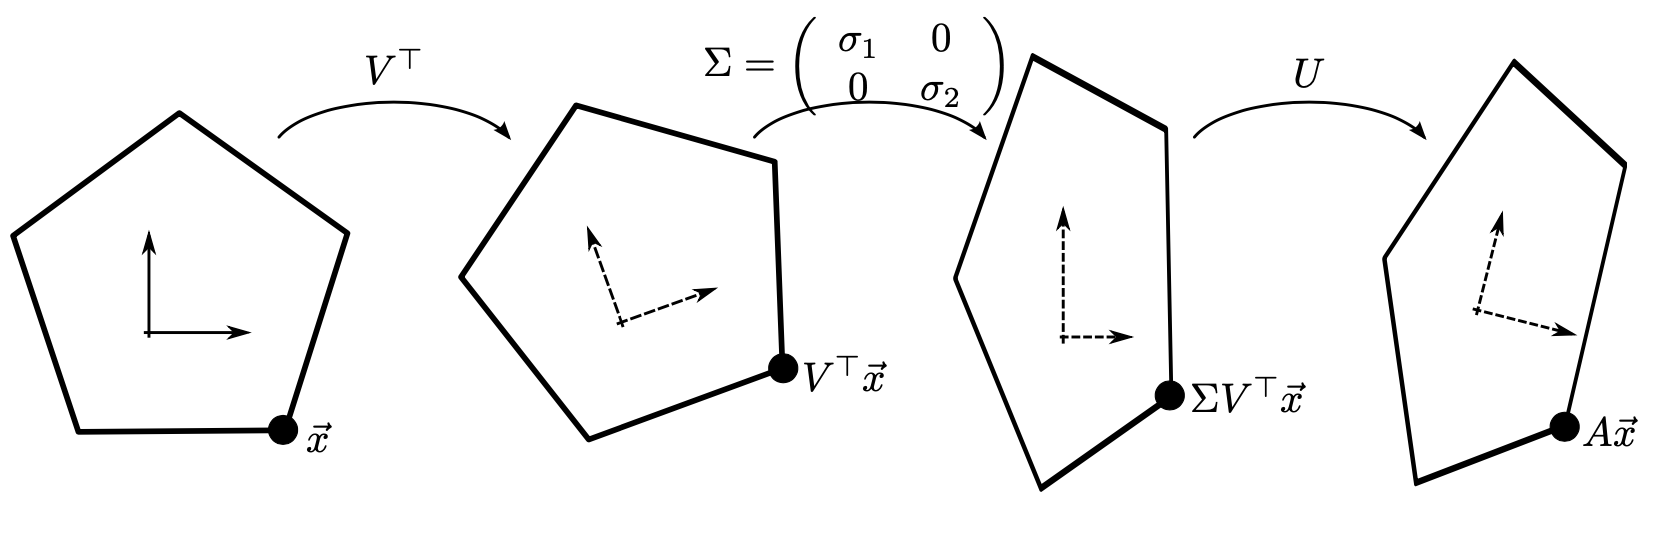
\includegraphics[width=4in]{Chapter1/geometric_svd.png}
  \caption{ Visually, for 2 by 2 matrices, one can see the SVD as a decomposition of the action of a matrix $\MA$ on vectors in $\R^2$ as being composed by a rotation, a stretching factor, and another rotation (also possibly reversing the orientation).}
\end{figure}

We continue to use the notation in the above proof, where the $\vu_i$ denote the columns of $\MU$ and $\vv_j$ denote the columns of $\MV$. Another often more convenient way to interpret the SVD is as follows.
If $\MU^\intercal \MA \MV = \Sigma$ for $\MA \in \mathbb R^{m \times n},$ then for $1 \leq i \leq n, \MA\vv_i = \sigma_i \vu_i$ and $\MA^\intercal \vu_i = \sigma_i \vv_i.$


\begin{proposition}
If $\MA \in \mathbb R^{m \times n},$ then $\norm{\MA}_2 = \sigma_1$ and $\norm{\MA}_{\Fro} = \sqrt{\sigma_1^2 + \ldots + \sigma_p^2}$
\end{proposition}

\begin{proof}
We present a proof of the second fact, leaving the first to the reader to confirm
$$\norm{\MA}_{\Fro} = \sqrt{\sum_{i,j} A_{i,j}^2} = \sqrt{\trace(\MA^\intercal\MA)} = \sqrt{\trace(\MV \Sigma \MU^\intercal \MU \Sigma \MV^\intercal)} = \sqrt{\trace(\MV \Sigma^2 \MV^\intercal)} $$
$$ = \sqrt{\trace(\MV^\intercal\MV \Sigma^2)} = \sqrt{\trace(\Sigma^2)} = \sqrt{\sigma_1^2 + \ldots + \sigma_p^2}$$
\end{proof}

It may be interesting to note that since orthogonal matrices preserve 2-norm distance, we have
$$\norm{\Sigma}_2 = \norm{\MU\MA\MV^\intercal}_2 = \norm{\MA}_2.$$

Recall the \define{kernel} of a matrix $\MA\in\R^{m\times n}$ is the set $\kernel(\MA) = \{\vv\in\R^n \ | \ \MA\vv = \vzero\}$ and the \define{image} of $\MA$ is the set $\image(\MA) = \{\MA\vv \ | \ \vv\in\R^n\}\subseteq \R^m$. Both the kernel and the image of $\MA$ are subspaces. The kernels and images of $\MA$ and $\MA^\intercal$ are often called the four fundamental subspaces of $\MA$. The reader should verify the following important result.
\begin{theorem}[Four Fundamental Subspaces]
If $\MA$ has $r$ positive singular values where $\MA = \MU\Sigma\MV^\intercal$ is an SVD for $\MA$, then $\rank(\MA) = r$ and 
$$\kernel(\MA) = \spann \{ \vv_{r+1}, \ldots, \vv_n \}$$
$$\image(\MA) = \spann \{ \vu_1, \ldots, \vu_r \}$$
$$\kernel(\MA^\intercal) = \spann \{ \vu_{r+1}, \ldots, \vu_m \}$$
$$\image(\MA^\intercal) = \spann \{ \vv_1, \ldots, \vv_r \}$$
\end{theorem}

Notice that the theorem indicates a fundamental conservation property about these fundamental subspaces. Specifically, 

\begin{corollary}[Rank-Nullity Theorem]
If $A \in \mathbb R^{m \times n}$, then 
$$dim(\kernel(\MA)) + dim(\image(\MA)) = n$$
$$dim(\kernel(\MA^\intercal)) + dim(\image(\MA^\intercal)) = m$$
\end{corollary}

\begin{proposition}
If $\MA \in \mathbb R^{m \times n}$, with $\rank(\MA) = r,$ then $\MA = \sum_{k = 1}^r \sigma_i \vu_i \vv_i^\intercal.$ 
\end{proposition}
\begin{proof}
$$\MA = \MU \Sigma  \MV^\intercal = \begin{bmatrix}
\vdots & \vdots & \vdots & \vdots & \vdots & \vdots \\
\sigma_1 \vu_i  & \ldots & \sigma_r \vu_r & 0 & \ldots & 0 \\
\vdots & \vdots & \vdots & \vdots & \vdots & \vdots
\end{bmatrix} \begin{bmatrix}
\ldots & \vv_1^\intercal & \ldots \\
& \vdots & \\
\ldots & \vv_n^\intercal & \ldots 
\end{bmatrix} = \sum_{i =1}^r \sigma_i \vu_i \vv_i^\intercal$$
\end{proof}

Adjusting the upper index of summation in the above formula turns out to have an interesting interpretation. The very useful matrix approximation theorem states that the matrix $\MA_k = \sum_{i=1}^k\sigma_i\vu_i\vv_i^\intercal$ is the closest approximation to the matrix $\MA$ among all matrices of rank $k$. This holds true for both the 2-norm and the Frobenius norm:
$$\MA_k = \underset{\rank(\MM) = k}{\argmin}||\MA - \MM||_\Fro$$
$$\MA_k = \underset{\rank(\MM) = k}{\argmin}||\MA - \MM||_2.$$
 
\section{Exercises}

\begin{enumerate}

    \item Consider the vector space $\CP_3(x) = \{a+bx+cx^2 \ | \ a,b,c,d\in\R\}$ consisting of polynomials $f(x)$ of maximum degree less than $3$. 
Consider the set $$\CB = \left\{1,\ -x+1,\ \frac{1}{2}(x^2-4x+2)\right\}$$
consisting of the first three Laguerre polynomials.
\begin{enumerate}
    \item Show that $\CB$ is a basis for $\CP_3(x)$. 
    \item Consider the map $E:\CP_3(x)\to\R^4$ by $$E(a+bx+cx^2) = [a, a-b, b-c,c]^\intercal$$
for a polynomial $a+bx+cx^2\in\CP_3(x)$. Show that the map $E$ is linear. 
\item Compute the matrix of $E$ with respect to the basis $\CB$ for $\CP_3(x)$ and the standard basis $\CB_\textnormal{std}$ for $\R^4$.
\item Determine the rank of $E$. Is $E$ invertible?
\end{enumerate}

\item \textbf{Examples of Positive Semi-Definite Matrices}

\begin{enumerate}
    \item Let $z \in \mathbb R^n$ be an $n$-vector. Show that $A = zz^T$ is positive semidefinite.
    \item Let $z \in \mathbb R^n$ be a non-zero $n$-vector. Let A = $zz^T$. What is the null-space of A? What is the rank of A?
    \item Let $A \in \mathbb R^{n \times n}$ be positive semidefinite and $B \in \mathbb R^{m \times n}$ be arbitrary, where $m, n \in \mathbb N$ Is $B A B^T$ Positive Semi-Definite? If so, prove it. If not, give a counterexample with explicit $A, B.$
\end{enumerate}



\item Let $\MU$ be an upper triangular matrix with with positive entries on its diagonal and define $\MA = \MU^\intercal\MU$. Use the matrix $\MU$ to define matrices $\ML$ and $\MD$ such that $\ML$ is lower unitriangular (lower triangular with $1$s along the diagonal), $\MD$ is diagonal with all positive entries, and $\MA = \ML\MD\ML^\intercal$. 

\item Let $\MA\in\mathbb{R}^{m\times n}$ where $m\geq n$, with SVD $$\MA=\MU\Sigma\MV^\intercal.$$
Express the column vector $\MA_{*,k}$ as a linear combination of the columns of $\MU$. That is, show that
$$\MA_{*,k}=\sum_{i=1}^n\beta_{i,k}\MU_{*,i}$$
and determine the coefficients $\beta_{i,k}$.
\end{enumerate}


\section{Solutions to Exercises}
\begin{enumerate}
    \item (a) To show that $\CB$ is a basis, suppose that $a+b(1-x)+c(\frac{1}{2}(x^2-4x+2)=0$ for some $a,b,c\in\R$. Then we have $(a+b+c)+(-b-2c)x+\frac{c}{2}x^2 = 0$ and we find that $a=b=c=0$.  This shows that $\CB$ is linearly independent. Now we can simply observe that since $\{1,x,x^2\}$ is a basis and $\CB$ is a linearly independent set with the same number of elements as $\{1,x,x^2\}$, $\CB$ must also be spanning and therefore a basis. (b) To show that $E$ is linear, take any polynomials $f,g\in\CP_3(x)$ and $a,b\in\R$. Write $f = f_0+f_1x+f_2x^2$ and $g = g_0+g_1x+g_2x^2$ where $f_i,g_j\in\R$ for all $i,j$. Then we observe that $E(af+bg) = E(a(f_0+f_1x+f_2x^2)+b(g_0+g_1x+g_2x^2)) = E(af_0+bg_0 + (af_1+bg_1)x + (af_2+bg_2)x^2) = [af_0+bg_0,a(f_0-f_1)+b(g_0-g_1),a(f_1-f_2)+b(g_1-g_2),af_2+bg_2]^\intercal = aE(f)+bE(g)$. (c) The matrix of $E$ with respect to $\CB$ and the standard basis for $\R^4$ is 
    $$
    \begin{bmatrix}
    E(1) & E(1-x) & E(\frac{1}{2}(x^2-4x+2)
    \end{bmatrix}
    =
    \begin{bmatrix}
    1 & 1 & 1\\
    0 & 2 & 3\\
    0 & -1 & -\frac{9}{2}\\
    0 & 0 & \frac{1}{2}
    \end{bmatrix}.
    $$
    (d) The columns of the matrix of $E$ are linearly independent and therefore the rank of $E$ is equal to the number of columns, so $\rank(E) = 3$. Since the matrix of $E$ is not square, $E$ is not invertible.

    \item \textbf{Fill In}
    \item Let $\MD = \diag(\MU)^2$. Then $\MD^{-1/2}\MU$ is upper unitriangular. Define $\ML = (\MD^{-1/2}\MU)^\intercal$. Then $\ML\MD\ML^\intercal = (\MD^{-1/2}\MU)^\intercal\MD(\MD^{-1/2}\MU) = \MU^\intercal(\MD^{-1/2})\MD\MD^{-1/2}\MU = \MU^\intercal\MU = \MA$.
    \item We have $\MA = \sum_{i=1}^r\sigma_i\vu_i\vv_i^\intercal$ so $\MA_{*,k} = \sum_{i=1}^n\sigma_i V_{i,k}\vu_i = \sum_{i=1}^n\sigma_i V_{i,k}\MU_{*,i}$ so we have $\beta_{i,k} = \sigma_i V_{i,k}$ for $1\leq i,j\leq n$.
\end{enumerate}